Human action recognition in video is a key technology for the development of a
wide variety of applications, such as surveillance, human-computer interaction,
and video annotation, among others. Consequently, it has received wide attention
in the computer vision community with a strong focus on recognition of atomic
actions in short video sequences
\cite{Aggarwal2011,Poppe2010,vishwakarma2013survey,weinland2011survey}.
As the area
evolves, there has been an increasing interest to develop more
flexible models that are able to operate on longer video sequences featuring
multiple concurrent or sequential actions, which we refer to as
\textit{complex actions}. Furthermore, in order to facilitate tasks such as
video tagging or retrieval, it is also highly appealing to provide these models
with capabilities to identify the spatial and temporal spans of each relevant
action. As an example, Figure \ref{fig:frontfigure} shows a potential usage
scenario, where an input video featuring a complex action has been automatically
provided with the set of labels, as well as, temporal and
spatial spans of its main atomic actions.

\begin{figure}[t]
\begin{center} \label{fig:frontfigure}
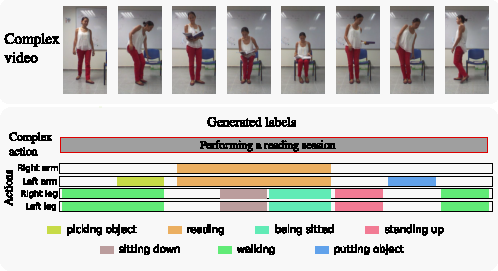
\includegraphics[width=0.98\linewidth]{Fig/portada.pdf}
%\fbox{\rule{0pt}{2in} \rule{0.9\linewidth}{0pt}}
%\includegraphics[height=0.28\linewidth]{jc/fig1_spatial.pdf}
%&
%\includegraphics[height=0.28\linewidth]{jc/fig1_temporal.pdf}\\
%(a) Spatial & (b) Temporal composition
\vspace{-0.5cm}
\end{center}
\caption{\footnotesize
Sample frames from a video sequence featuring a complex action. 
Our method is able to identify the complex action, as well as, the temporal and 
spatial span of meaningful atomic actions (actionlets) and local body part 
configurations (motion poselets).}
\vspace{-0.5cm}
\end{figure}

A promising direction is that of incorporating human body pose information
to enable such detailed reasoning about complex actions.
While generic human body pose estimation from color images remains difficult,
the emergence of cost-effective RGB-D cameras has enable robust
algorithms for body pose estimation from depth images
\cite{Shotton:EtAl:11}, and these sensors are now
a reliable source to obtain 3D joint positions of the human skeleton. 
As it has been noticed long ago \cite{Johansson:1973}, the use of human body
pose cues is highly informative to discriminate among human actions.
Furthermore, recent action recognition methods have
showcased the relevance of joint position information to 
recognize actions \cite{Jhuang2013,Wang2013}. We believe that the 
inherent
hierarchical and compositional relations among joint positions, body poses, and 
actions, is behind the recent success of models that exploit these 
relations to achieve action recognition.

In this work, we present a new pose-based approach to recognize
complex human actions in videos. As a distinguishing feature,
given a video featuring a complex action, the
proposed method is able to identify not only the complex action occurring in the
video, but also the temporal and spatial extent of the corresponding atomic
actions. In terms of spatial extent, each atomic action is characterized by a 
set of characteristic local body configurations. In particular, we focus on 
actions that can be characterized by the
body motions of a single actor, such as running, drinking, or eating. This
allows us to test our approach using several popular benchmark datasets.

Our model follows previous hierarchical compositional approaches based on Bag
of Words (BoWs) representations, such as \cite{Wang2013, 
Lillo2014,Taralova:EtAl:2014,Tao2015}.
Briefly, these models learn local dictionaries that capture
appearance and motion patterns of different body parts. We refer to these local 
patterns as motion poselets \cite{Bourdev:EtAl:2010, Tao2015}. These
dictionaries are then used to construct BoW representations for the training
videos, that in turn are used to learn action classifiers.
We formulate learning as an energy minimization
problem, where structural hierarchical relations are modeled by sub-energy
terms that constraint compositions among
motion poselets and actionlets, as well as, their spatial and 
temporal relations.

Our model has some key novel properties with respect to previous work.
Our model infers \emph{both at test and training time},
action labels for each detected motion poselet, as 
well as, its temporal and spatial span. To achieve this, we introduce a novel 
formulation based on a structural latent SVM model \cite{Yu:Joachims:2010} and a 
initialization method based on self-pace learning \cite{Kumar:EtAl:2010}. 
Furthermore, we extend the pose dictionary learning process to the level of 
atomic actions by learning for each action a set of classifiers that are able to 
capture relevant variations in its execution. We refer to the component of these 
dictionaries of action modes as actionlets \cite{Wang2012}. Finally, given 
that we are dealing with long videos, where it is possible to find idle spatial 
or temporal parts, we include in our model a mechanism that identifies and 
discards idle or non-informative body parts, we refer to this mechanism as 
garbage collector. In summary, this work makes the following main 
contributions.
\emph{(1)}Motion poselets: at training time our hierarchical model includes a 
new semi-supervised mechanism to learn dictionaries of relevant body 
part configurations or motion poselets. A test time our model is able to 
automatically infer the presence and temporal span of each motion poselet.
%\emph{(2)}Actionlets: our hierarchical model includes a 
%semi-supervised mechanism to infer dictionaries of relevant body 
%part configurations or motion poselets.
\emph{(2)}Actionlets: our hierarchical model includes a 
semi-supervised mechanism to infer dictionaries of relevant action modes or actionlets.
\emph{(3)}Garbage collector: our model includes a mechanism that
selectively filter-out noisy and irrelevant spatial and temporal areas of the
input videos.
\emph{(4)}Empirical evidence indicating that the 
combination of the previous
contributions in a single hierarchical model result in a more informative and 
accurate solution than previous state-of-the-art approaches.

In the rest of the paper we review related previous work
(Sec.~\ref{sec:related_work}),
describe the proposed method
(Sec.~\ref{sec:model}),
present qualitative and quantitative experiments
on benchmark datasets
(Sec.~\ref{sec:experiments});
and close with conclusions (Sec.~\ref{sec:conclusions}).
